
%%% Local Variables:
%%% mode: latex
%%% TeX-master: t
%%% End:

\chapter{引言}
\label{cha:intro}


\section{选题背景}
\label{sec:background}

21世纪的最初十年是计算机技术与互联网应用发展极为迅速的时期。在此期间,人们见证了CPU主频步入GHz时代,内存的容量和吞吐率按部就班地翻番,硬盘容量进入了TB级,人们探索互联网的接入方式也从曾经的56kbps甚至更慢的modem换成了带宽以Mbps计的宽带接入。可以说,这些都为数字多媒体技术在计算机和互联网上的应用奠定了硬件基础。

我们从十年前看VCD,五年前看DVD,到现在拥有了720p到1080p的高清电影资源;从8bit的音频到24bit、192kHz采样的无损音乐格式,无不需要计算能力更强和存储容量更大的计算机来处理。信息化的大步跨越让多媒体技术在我们日常生活中扮演越来越重要的角色。各种新的应用也接踵而来。

%3D电视的发展
3D电视经过多年的发展,已经逐渐走向成熟。在CES(Consumer Electronics Show) 2010的展厅里,“3D”成了最大的赢家,备受关注。Panasonic的VT25平板3D电视也获得了这届CES的“Best in Show Award”。无论是各大家电厂商展台上的3D电视,还是可以用在现有系统上的nVidia 3D Vision套装,都令消费者们感受到了3D时代即将来临。其实,3D电视的起源并不比2D电视晚很长时间\cite{smolic2007coding},但是由于其对计算、存储和传输的资源消耗比普通2D电视高出一倍甚至数倍,所以一直以来未能普及。

%3D视频编码的发展
为了满足资源有限条件下的3D视频应用,各种编码技术陆续诞生,以一定量的比特率来描述多视频信号,达到一定的压缩率,同时尽可能减小失真。在这个过程中,国际标准化组织应运而生。目前国际上有两个音视频编码标准化组织:
\begin{itemize}
\item 一是国际电信联盟标准化组(ITU-T)下属的视频编码专家组(VCEG:Video Coding Expert Group)。制定了一系列视频通信协议和标准,包括H.261、H.263、H.263+、H.264等。主要应用在视频通信领域,如视频会议等。
\item 二是国际标准化组织(ISO)和国际电工委员会(IEC)下属的运动图像编码专家组(MEPG:Motion Picture Expert Group)。自1988年成立以来,研究和开发了多种多媒体压缩标准,包括MPEG-1、MPEG-2、MPEG-4、MPEG-7等。主要应用在存储媒介(DVD)、广播电视网、有流媒体传输等。
\end{itemize}
\begin{figure}[htbp]
\begin{center}
	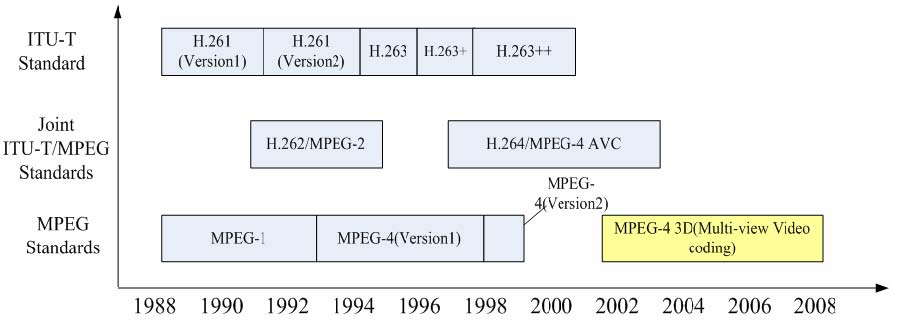
\includegraphics[width=\textwidth]{codecroadmap.jpg}
\caption{MPEG、VCEG、JVT视频编解码标准的发展}
\label{fig:codecroadmap}
\end{center}
\end{figure}

在2001年6月,经过评估发现,H.26L编码技术基本能够满足MPEG的标准需求,因此MPEG与VCEG的成员共同成立了一个新的工作组JVT(Joint Video Team),来推动和管理H.26L的最后标准化开发,并在2003年形成了视频标准,同时被MPEG和VCEG采纳:MPEG将其定为MEEG-4 part 10,VCEG将其定为H.264。MPEG和VCEG制定的主要标准见。H.264/MPEG-4 part 10标准称为高级视频编码(AVC:Advanced Video Coding),扩展性较好,用于3D视频的多视点视频编解码(MVC:Multi-view Video Coding)就是其一个扩展。

MVC通过将多个设备采集到的视频同时编码,利用时间和各个视角间视频信号的统计相关性,设计一种预测机制,令描述视频所需的比特率比单独压缩各路信号更低。这个方法在提高视频编码压缩率的同时,增加了编解码的复杂度,要求处理更大量的数据和进行更多的计算。

\section{已有工作}
\label{sec:previouswork}

%MVC Decoder工作

%庞一等 论文

\section{需求分析}
\label{sec:requirements}

%从应用层面分析需求

\section{毕设任务介绍}
\label{sec:workbrief}

%列举毕设任务